%\documentstyle[10pt,twoside]{article}
%\documentstyle[twoside]{article}
\documentclass[twoside]{article}
\setlength{\oddsidemargin}{0.25 in}
\setlength{\evensidemargin}{-0.25 in}
\setlength{\topmargin}{-0.6 in}
\setlength{\textwidth}{6.5 in}
\setlength{\textheight}{8.5 in}
\setlength{\headsep}{0.75 in}
\setlength{\parindent}{0 in}
\setlength{\parskip}{0.1 in}

\usepackage{graphicx}
\usepackage{url}

%
% The following commands sets up the lecnum (lecture number)
% counter and make various numbering schemes work relative
% to the lecture number.
%
\newcounter{lecnum}
\renewcommand{\thepage}{\thelecnum-\arabic{page}}
\renewcommand{\thesection}{\thelecnum.\arabic{section}}
\renewcommand{\theequation}{\thelecnum.\arabic{equation}}
\renewcommand{\thefigure}{\thelecnum.\arabic{figure}}
\renewcommand{\thetable}{\thelecnum.\arabic{table}}
\newcommand{\dnl}{\mbox{}\par}

%
% The following macro is used to generate the header.
%
\newcommand{\lecture}[4]{
   \pagestyle{myheadings}
   \thispagestyle{plain}
   \newpage
   \setcounter{lecnum}{#1}
   \setcounter{page}{1}
   \noindent
   \begin{center}
   \framebox{
      \vbox{\vspace{2mm}
    \hbox to 6.28in { {\bf CMPSCI~677~~~Operating Systems
                        \hfill Spring 2018} }
       \vspace{4mm}
       \hbox to 6.28in { {\Large \hfill Lecture #1: #2  \hfill} }
       \vspace{2mm}
       \hbox to 6.28in { {\it Lecturer: #3 \hfill Scribe: #4} }
      \vspace{2mm}}
   }
   \end{center}
   \markboth{Lecture #1: #2}{Lecture #1: #2}
   \vspace*{4mm}
}

%
% Convention for citations is authors' initials followed by the year.
% For example, to cite a paper by Leighton and Maggs you would type
% \cite{LM89}, and to cite a paper by Strassen you would type \cite{S69}.
% (To avoid bibliography problems, for now we redefine the \cite command.)
%
\renewcommand{\cite}[1]{[#1]}

% \input{epsf}

%Use this command for a figure; it puts a figure in wherever you want it.
%usage: \fig{NUMBER}{FIGURE-SIZE}{CAPTION}{FILENAME}
\newcommand{\fig}[4]{
            %\vspace{0.2 in}
            \centerline{\includegraphics[scale=#2]{#4}}
            \begin{center}
            Figure \thelecnum.#1:~#3
            \end{center}
    }

% Use these for theorems, lemmas, proofs, etc.
\newtheorem{theorem}{Theorem}[lecnum]
\newtheorem{lemma}[theorem]{Lemma}
\newtheorem{proposition}[theorem]{Proposition}
\newtheorem{claim}[theorem]{Claim}
\newtheorem{corollary}[theorem]{Corollary}
\newtheorem{definition}[theorem]{Definition}
\newenvironment{proof}{{\bf Proof:}}{\hfill\rule{2mm}{2mm}}

% Some useful equation alignment commands, borrowed from TeX
\makeatletter
\def\eqalign#1{\,\vcenter{\openup\jot\m@th
  \ialign{\strut\hfil$\displaystyle{##}$&$\displaystyle{{}##}$\hfil
      \crcr#1\crcr}}\,}
\def\eqalignno#1{\displ@y \tabskip\@centering
  \halign to\displaywidth{\hfil$\displaystyle{##}$\tabskip\z@skip
    &$\displaystyle{{}##}$\hfil\tabskip\@centering
    &\llap{$##$}\tabskip\z@skip\crcr
    #1\crcr}}
\def\leqalignno#1{\displ@y \tabskip\@centering
  \halign to\displaywidth{\hfil$\displaystyle{##}$\tabskip\z@skip
    &$\displaystyle{{}##}$\hfil\tabskip\@centering
    &\kern-\displaywidth\rlap{$##$}\tabskip\displaywidth\crcr
    #1\crcr}}
\makeatother

% **** IF YOU WANT TO DEFINE ADDITIONAL MACROS FOR YOURSELF, PUT THEM HERE:



% Some general latex examples and examples making use of the
% macros follow.

\begin{document}

%FILL IN THE RIGHT INFO.
%\lecture{**LECTURE-NUMBER**}{**DATE**}{**LECTURER**}{**SCRIBE**}
\lecture{22}{April 18}{Srinivasan Iyengar}{\textbf{Suhas Keshavamurthy}}

\section{Introduction}

This lecture covered topics related to Pervasive Computing, Internet of Things and Smart Buildings

\section{Pervasive Computing}

Computing is becoming more ubiquitous (sensing and computing 'Everywhere'). One of the popular examples of this is Smartphones. \\
A lot sensors are also embedded in many physical environments like buildings. For example : PIR sensor is used to detect when a person has entered a room and switch on the lights 

\subsection{Rise of Pervasive Computing}
The rise of pervasive Computing has been possible due to 
\begin{itemize}
    \item Miniaturization of Computing : Sensors have become tiny in terms of physical dimensions. This is particularly true with the growth of MEMS (Microelectromechanical systems) technology. A MEMS sensor can transform mechanical, thermal, biological, chemical, optical, and magnetic phenomena into electrical signals. In future it is likely that sensor sizes will reduce to nano-scale dimensions. 
    \item Internet of Things(IoT) : This is nothing but a network of physical devices which are able to talk to each other and then trasfer data to the cloud.
\end{itemize}

\subsection{Applications}

\subsubsection{Smart Health}
Early wearable devices were able to track heart rate, number of steps etc for the purpose of fitness, exercise tracking and monitoring sleep. Fitbit is the most popular example of such a wearable device.
Newer technology does much more than this. For example: Smart Clothing - Devices embedded in the clothing are able to do on-body monitoring for sweat detection etc. Smart glasses are able to track gaze in order to detect fatigue.

\subsubsection{Smart Buildings}
Some of the examples of devices that make building infrastructure smarter include Thermostat, Smart Plugs, Smart appliances, Smart Lock etc.
A Smart appliance like a smart-fridge is potentially able to detect food spoilage etc. Nest Thermostats are examples of smart thermostats that can learn usage pattern and dynamically control temperature settings. These devices can be controlled through a phone or voice interface.
\begin{center}
    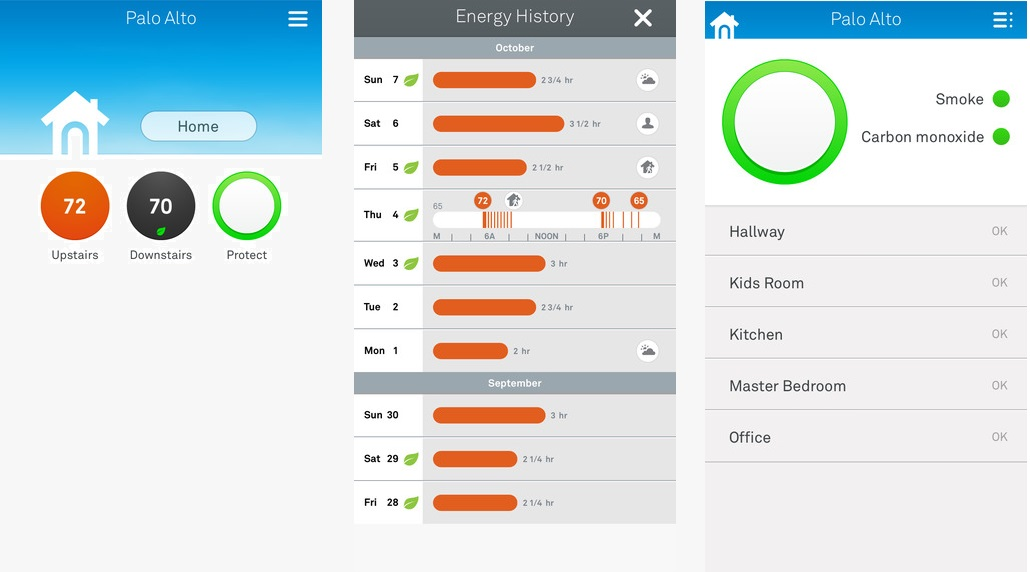
\includegraphics[scale=0.5]{nest-thermostat.jpeg}
\end{center}

\subsubsection{Smart Transportation}
One of the major examples of smart transportation are \textit{Connected Cars}. Potential applications include Accident avoidance (pedestrian detection etc.), fleet management (cars can start/stop at the same time) and real-time public transport alerts.

\subsubsection{Smart Roadways}
Sensors can be used to switch on street lighting only if an automobile is passing nearby or dynamically direct cars to different lanes. They can also be used to monitor road conditions and for the purposes of Traffic management. For Ex: Austin has a program where signals from Bluetooth-enabled cars are used to estimate traffic density in the streets.

\subsection{Design of 'Smart Infrastructure'}
A typical application includes a personal device that is able to communicate with a mobile phone over a low-power network channel. The mobile phone then uploads the data to the cloud. In the cloud, the server performs analytics on the data and may provide feedback to the phone.

Another possible design is where the sensors in the environment upload data directly to the cloud. Ex: Smart Energy meters

Different elements of a distributed network of resource-constrained smart devices (also referred to as sensor nodes) are as follows -  
\subsubsection{CPU}
The sensor nodes have very small CPU's. Popularly used CPU's are \textit{Atmel AVR} (8-bit instruction set, 128 KB on-chip flash, ~8 mA current draw) and \textit{TI MSP430} (16-bit instruction set, 10 KB RAM, 48 KB flash, ~2 mA current draw). As silicon technology evolves, the trend is for more compute to be available with lower energy consumption. Thus newer CPU's for these applications include \textit{ARM 7} (32 bit, 50 MHz, 1 MB RAM), \textit{ARM 9} etc

\begin{center}
    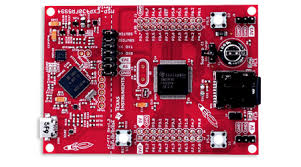
\includegraphics[scale=0.5]{msp430.jpeg}   
    \captionof{}{MSP430 board}
\end{center}


\subsubsection{Low-Power Radios}
Communication is essential for a network of nodes to work together. The ISM Band (Industrial Scientific and Medical Band) is free for applications to communicate and is unlicensed. Some of the commonly used spectrum is 2400 MHz for Bluetooth and 900 MHz (33cm). \\
Different radio communication protocols work through different means. Zigbee (IEEE 802.15.4) works by modulating phase and Bluetooth (IEEE 802.15.1) works by modulating frequency of radio waves.
These communication protocols typically have practical ranges of less than 100 meters. Chipcon CC2420 is a popular radio chipset. \\
An essential requirement of these radios is low power. Typically in these radios the energy consumption is higher while receiving than transmitting. This is because the radio needs to be 'ON' all the time, while it can transmit for a short time and go to sleep.

\subsubsection{Battery Power}
Battery Power is a big concern in IoT. For example: A Mica 2 "mote" has a battery capacity of 2500 mAH. The mote consumption is around 25 mA which gives it a lifetime of 100 hours. In order to extend the life of the node, following are possible alternatives
\begin{itemize}
    \item Bigger Battery : More capacity
    \item Energy Harvesting : Charge the battery in the node or use energy directly from the environment through sources like Solar, Wind or motion
    \item Duty Cycling : Switch on and off the mote at a particular frequency based on the application
\end{itemize}


\subsubsection{Sensors}
The sensors in the system are responsible for measuring external phenomena. They can be used to measure temperature, humidity, light, acoustics, location etc. For example : the phone screen brightness is adjusted based on ambient light. \\
Sensor fusion is the technique of deriving insights by fusing data from multiple sensors. Another challenge is sensor placement. The multiple sensors need to placed so that they can cover the entire area that needs to be monitored and provide redundancies in case of failure.
Apart from the use of batteries, it is possible for sensors to havest energy from the environment to power themselves. 

\subsection{Typical Design Issues}

The typical concerns while building a pervasive computing systems are :
\begin{itemize}
    \item Node : Maximize the lifetime of the node by increasing the battery power through various techniques
    \item Network of Sensors : The data from various kinds of sensors need to be aggregated together. Localization and synchronization among the nodes in the network based on signal strength, direction etc is also important. Another concern is the protocol for routing of the communication from one node to another
    \item Server Side Processing : On the server, we can employ big-data analytics in order to derive insights from the data and provide recommendations and alerts.
\end{itemize}

\section{Green Computing}
There are two major aspects of Green Computing
\begin{itemize}
    \item Greening of Computing : Here the attempt is to design energy-efficient hardware, software and systems.
    \item Computing for Greening : It is the use of computers to make physical infrastructure more efficient.
\end{itemize}

\subsection{Historical Overview}
Historically the necessity for better energy efficiency has been driven by the need for energy-efficient mobile devices where the motivation has been longer battery life, and growth of data center where the motivation has been to lower the electricity costs. 
Green computing is also important in order to lower the carbon footprint and to improve efficiency of other systems.
The typical \textit{compute} energy consumption is 20\% in an office building, 50-80\% at a large university. It is 3\% of total energy consumption today and is growing rapidly.

\subsection{Data Centers}
A data center is a facility for housing a large number of servers and data. For example: A Google data center can be many football fields big, housing more than 100000 servers and consuming 100 MW of electricity.
The energy cost of running a data center is very high. PUE or Power Usage Effectiveness is the ratio of total energy consumed by a data center to the energy delivered for compute. Typical PUE is between 1.5 - 2. A PUE of 2 indicates that the energy cost to run the data center is twice that of delivering power to the servers. Google achieves a PUE of 1.2 which is an indication of high efficiency of Google data center infrastructure. \\
\begin{center}
    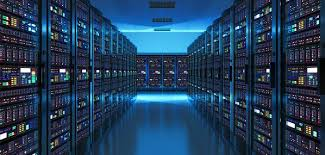
\includegraphics[scale=0.5]{data_center.jpeg}    
\end{center}

\subsection{Greening of Computing}
Following are the considerations while designing computing systems that are more energy efficient.
\begin{itemize}
    \item Reduce Server Cost : This is done by purchasing more energy-efficient hardware including servers, power supplies etc. In certain cases it is more efficient to run the data center through DC rather than AC.
    \item Server Management : The power cost can be reduced by intelligent power management of servers by turning them off while not in use; use of virtualization by moving applications to a concentrated number of physical machines running virtual instances. 
    \item Cooling Cost : This would involve design of better air-conditioning, thermal engineering and innovative methods of cooling like moving data-centers to cold places like Ireland etc.
    \item Desktop management : In large companies with thousands of desktops, IT tasks like update, virus scan are generally scheduled during the nighttime. Automatic sleep and wakeup policies enable better desktop power management and reduce overall power consumption.
\end{itemize}

\subsection{IT for Greening}
Modern buildings have a distributed system of nodes. They are used to perform the following actions 
\begin{itemize}
    \item Monitoring by Sensors : Energy consumption in the building can be monitored at the outlet-level or meter-level.
    \item Analyzing the data : Real-time usage data is provided by the energy monitors/sensors to the Building Management System (BMS). This data can be used for modeling, analytics and prediction using statistical techniques and ML. In a residential setting, smart thermostats like \textit{Nest} can learn household patterns by collecting energy usage and temperature data over a period of time.
    \item Use of Renewables : There has been a significant growth of renewable energy adoption including Rooftop wind turbines, solar PV installation and solar thermal power. One of the challenges in the usage of renewable energy is that it is intermittent in nature and is influenced by rapidly changing external environmental conditions like cloud cover, temperature etc. 
    \item Forecasting of renewable energy : The challenge is to design predictive analytics in order to model and forecast energy generation. One of the use case of forecasting is in EV charging stations. Solar panels are installed in parking lots, rest areas and garages. Intelligence is required to design charging schedules to address questions like \textit{when to charge? Which EV to charge? and by How much?}
\end{itemize}
The data can also be used to motivate consumers to be more energy efficient as well as reveal insights into usage patterns, cause of wastage and improve efficiency.

\end{document}
